\section{\color{blue}{Trajectory planning for interception with terminal constraints}}
%%%%%%%%%%%%%%%%%%%%%%%%%%%%%%%%%%%%%%%%%%%%%%%%%%%%%
\begin{frame}[noframenumbering]
	\tableofcontents[currentsection]
	The guidance-related work presented here was carried out under the AR\&DB sponsored project
	“Multi-Vehicular Cooperative Pursuit and Evasion Guidance Strategies: Multi-Agent Perspective”
	(2022–2024)

	\color{magenta}{Principal Investigator: Prof. Shashi Ranjan Kumar}, Department of Aerospace Engineering, IIT Bombay
\end{frame}
%%%%%%%%%%%%%%%%%%%%%%%%%%%%%%%%%%%%%%%%%%%%%%%%%%%%
\begin{frame}{Problem Statement}
	\vspace{-0.5cm}
	%\begin{alertblock}{}
	%Consider a planar interceptor-target engagement geometry as shown. Given an interceptor's launch angle ($\gamma_M$), (constant) speed ($V_M$ ), initial range-to-go ($r$), and maximum lateral acceleration capability ($a^{\rm max}$), design a simple, easy-to-implement guidance law that meets the desired impact/approach angle ($\gamma_T$) and impact/terminal time ($t_{imp}$) requirements.
	%\end{alertblock}
	%\vspace{-0.5cm}
	\begin{figure}
		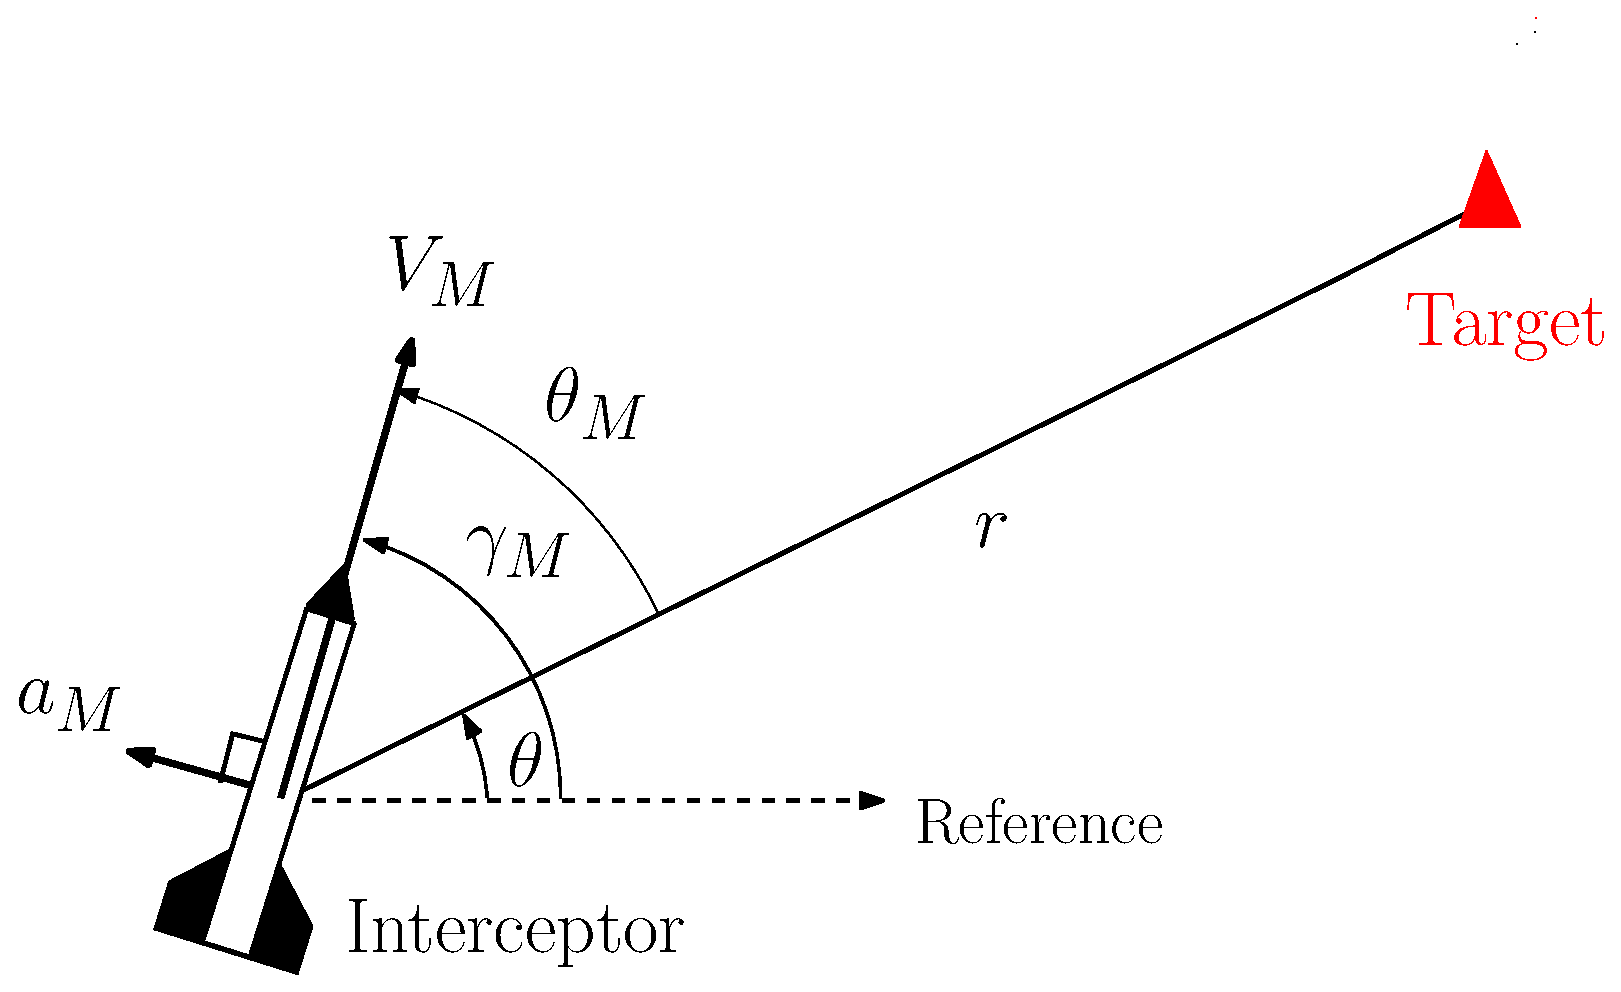
\includegraphics[scale=0.33, keepaspectratio]{Images/dubins_eng.eps}\\
		% \label{ChainLeader}
		% \caption{Engagement scenario against a stationary target.}
	\end{figure} 
	%\vspace{-0.5cm}
	\begin{columns}[T]
		\begin{column}{0.46\textwidth}
			%\column{0.46\textwidth}
			-- \textbf{Geometry: }Planar Engagement\\    
			-- \textbf{Known Parameters: }Launch Angle, Initial Range, Maximum Lateral Acceleration, Speed, \textcolor{red}{Desired Impact Angle and Time}
		\end{column}
		\vrule{}
		\begin{column}{0.5\textwidth}
			%\column{0.5\textwidth}
			-- \textbf{Assumption: } $\theta=0$ \\
			-- \textcolor{blue}{\textbf{Objective: }Design a simple and easy-to-implement guidance law to satisfy the terminal constraints}    
		\end{column}
	\end{columns}
	%\begin{alertblock}{}
	%   We'll consider $\theta=0$ i.e. the target and the launching platform are in the same reference plane. This implies $\gamma_M=\theta_M$ and $\gamma_T=\theta_T$
	%\end{alertblock}
\end{frame}
%%%%%%%%%%%%%%%%%%%%%%%%%%%%%%%%%%%%%%%%%%%%%%%%%%%%%%%%%%%%%%%%%%%%%%%%%%%%%%%%%%%%%%%%%%%%%%%%%
\begin{frame}{Introduction: Why Terminal Constraints Are Important?}
	\begin{figure}
		\centering
		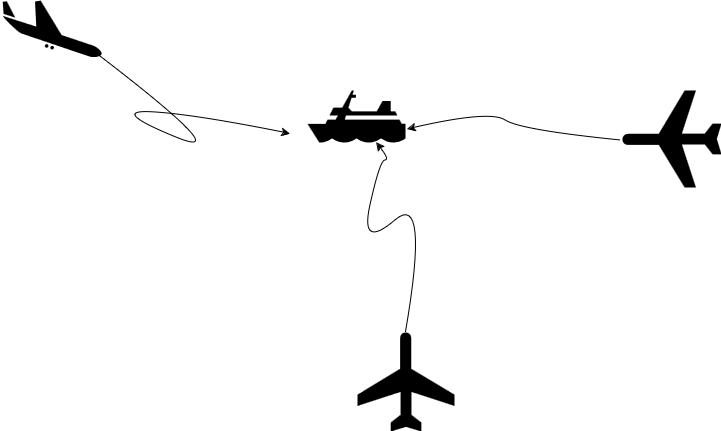
\includegraphics[scale=0.25]{Images/basicattack.png}
	\end{figure}
	\begin{columns}[T]
		\begin{column}{0.59\textwidth}
			%\column{0.46\textwidth}
			-- Exploit the geometric vulnerability\\    
			-- Enhancing warhead effectiveness \\
			-- Exploit fan-shaped coverage zones of radars
		\end{column}
		\vrule{}
		\begin{column}{0.41\textwidth}
			%\column{0.5\textwidth}
			-- Counter defense systems \\
			-- Achieve salvo attack \\
			-- Improve hit-to-kill probability 
		\end{column}
	\end{columns}
	\begin{alertblock}{Simultaneous Control}
		-- Challenging \quad \quad     -- Scarcely examined in the literature
	\end{alertblock}
\end{frame}
%%%%%%%%%%%%%%%%%%%%%%%%%%%%%%%%%%%%%%%%%%%%%%%%%%%%%%%%%%%%%%%%%%%%%%%%%%%%%%%
\begin{frame}{Definitions}
	\begin{defi}[Impact Angle]
		The angle between the velocity vectors of the two adversaries (target and interceptor) at the instant when interception of the target by the interceptor occurs. 
		
		For stationary targets, the impact angle is defined as the angle between the interceptor's velocity vector and some well-defined reference.
	\end{defi}
	\begin{defi}[Impact Time]
		The total time taken after the launch of the interceptor to intercept the target.$$t_{\rm imp}= t_{\rm el} + t_{\rm go},$$ where $t_{\rm el}$ is the time elapsed since the interceptor has been launched, and $t_{\rm go}$ is the time-to-go, i.e., the expected time remaining till interception occurs.
	\end{defi}
\end{frame}

%%%%%%%%%%%%%%%%%%%%%%%%%%%%%%%%%%%%%%%%%%%%%%%%%%%%%
\begin{comment}
\begin{frame}{Dubins Path (1957)\footnotemark[1]}
	\vspace{-0.5cm}
	\begin{columns}[T]%beamer
		\column{0.5\textwidth}
		\begin{defi}
			\justifying
			The shortest curvature bounded path (i.e. $a_M<a_{max}$) between two oriented points is given by a geometric pattern $CCC$ or $CSC$ or a subset of either.
			\begin{itemize}
				\item CSC=$\{LSR, RSL, LSL, RSR\}$
				\item CCC=$\{LRL, RLR\}$
			\end{itemize}
			$C$ - denotes a circular path \\
			$L,R$ - denotes the left and right turning circular paths, respectively. \\
			$S$ - denotes a straight path with zero curvature, i.e., $a_M=0$
		\end{defi}
		\vrule{}
		\column{0.5\textwidth}
		\begin{figure}
			\centering
			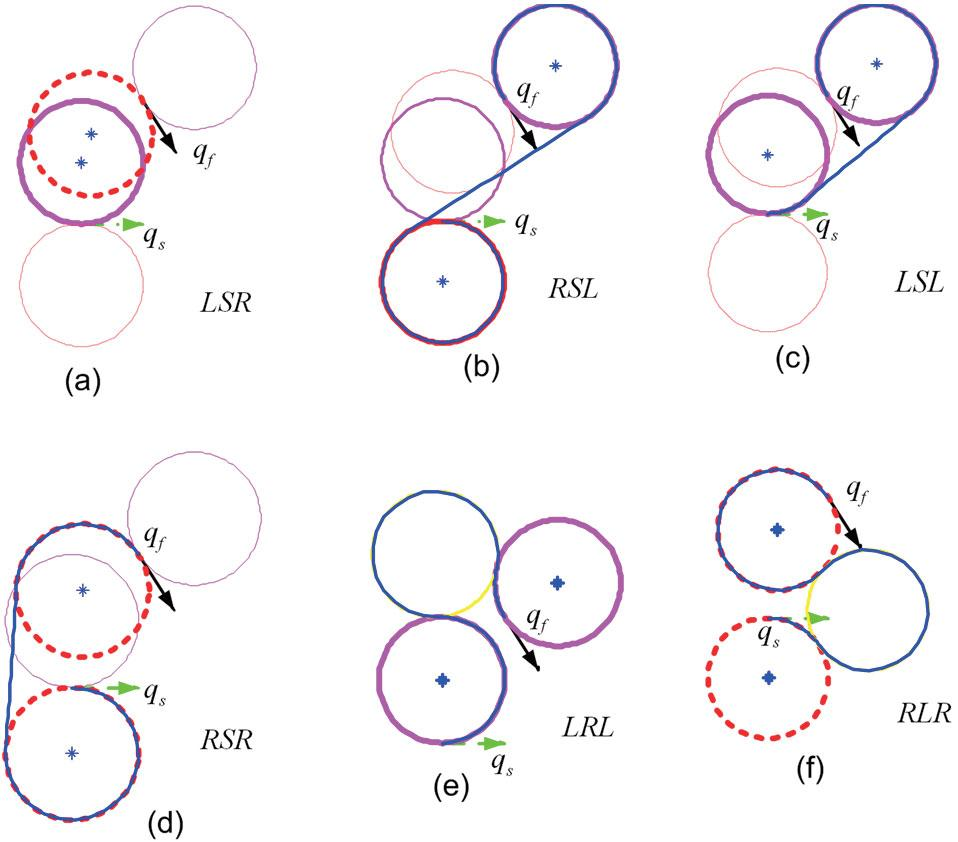
\includegraphics[scale=0.5,width=0.8\textwidth]{Images/dubin.jpeg}
		\end{figure}
	\end{columns}
	\vspace{-0.5cm}
	\footnotetext[1]{Dubins, Lester E. "On curves of minimal length with a constraint on average curvature, and with prescribed initial and terminal positions and tangents." American Journal of mathematics 79.3 (1957): 497-516.}
	\footnotetext[2]{PicSource: I. A. Hameed, "Coverage path planning software for autonomous robotic lawn mower using Dubins' curve," 2017 IEEE International Conference on Real-time Computing and Robotics (RCAR), Okinawa, Japan, 2017, pp. 517-522}
\end{frame}

\end{comment}
%%%%%%%%%%%%%%%%%%%%%%%%%%%%%%%%%%%%%%%%%%%%%%%%%%%%%%%%%%%%%%%%%%%%%%%%%%
\begin{frame}{Dubins Type CLC Path }
	\begin{figure}
		\centering
		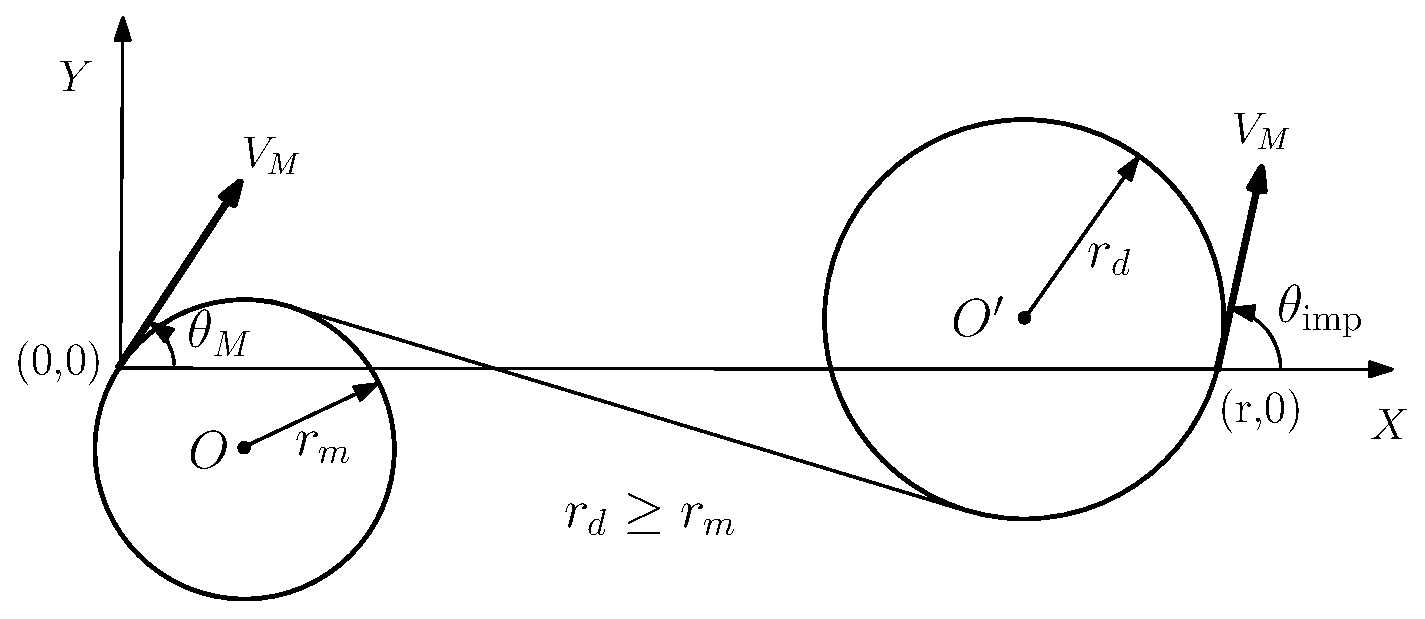
\includegraphics[width=0.4\textwidth, keepaspectratio]{Images/fig1.eps}\\
		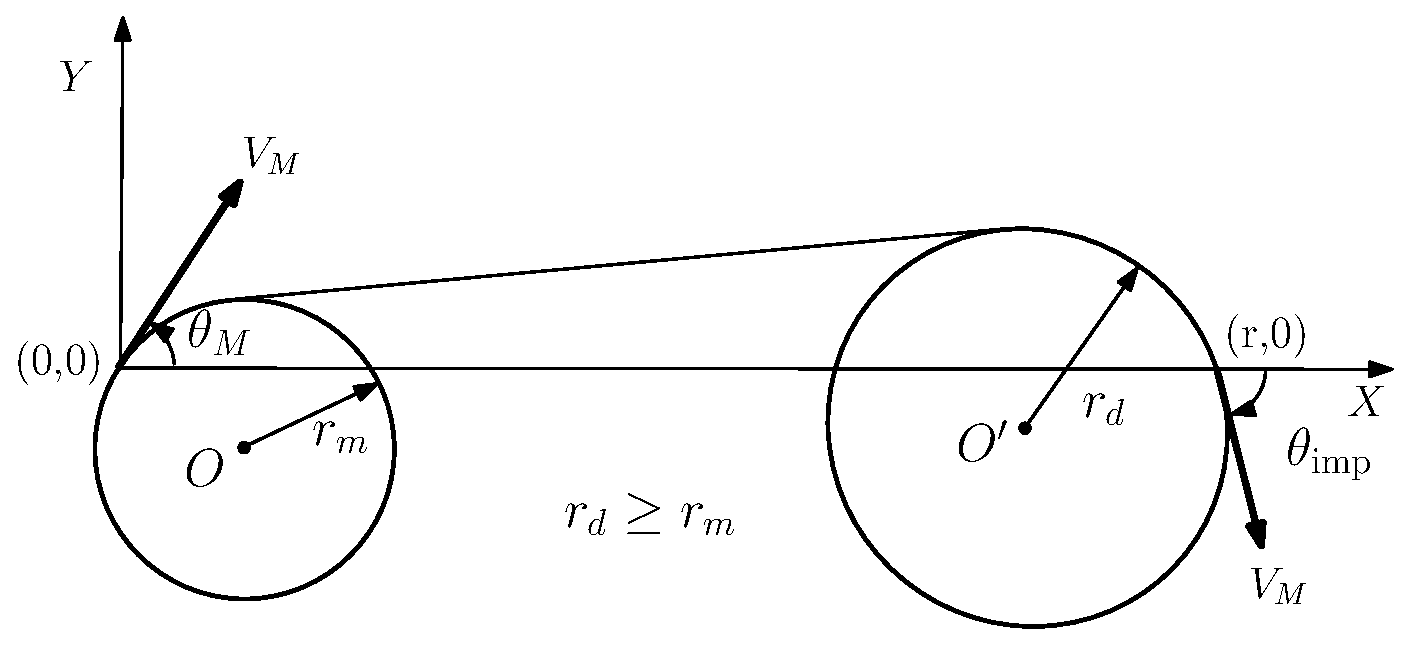
\includegraphics[width=0.4\textwidth, keepaspectratio]{Images/fig2.eps}
		%\caption{Dubins like path with Trasverse Common Tangent (TCT ) and Direct  Common Tangent (DCT)}
	\end{figure}
	%\vspace{-0.5cm}
	%\begin{columns}[T]
	%\column{0.46\textwidth}
	-- TCT based analysis \\    
	-- $C_1$- Constant radius,$C_2$- Variable radius, our design parameter\\
	-- Bounds on TCT and DCT
	%\vrule{}
	%\column{0.5\textwidth}
	%-- \textbf{Assumption: } $\theta=0$ \\
	%-- \textcolor{blue}{\textbf{Objective: }Design a simple and easy-to-implement guidance law to satisfy the terminal constraints}
	%\end{columns}
	%\begin{alertblock}{Note:}
	%   \begin{itemize}
		%      \item In this analysis, we will focus solely on the TCT-based path, as other analyses can be performed similarly and yield nearly identical results.
		%     \item We will maintain the radius of the first circle equal to the minimum turn radius, while using the radius of the second circle as a design parameter to adjust the path length to achieve the desired impact time.
		%    \item The TCT ceases to exist when the circles touch each other, whereas the DCT ceases to exist when one circle is contained within the other.
		% \end{itemize}
	%\end{alertblock}
\end{frame}
%%%%%%%%%%%%%%%%%%%%%%%%%%%%%%%%%%%%%%%%%%%%%%%%%%%%%%%%%%%%%%%%%%%%%%%%%%%%%%%%%%%%%%%%%%%%%
\begin{frame}{TCT Based Path Planning}
	\vspace{-0.3cm}
	\begin{figure}
		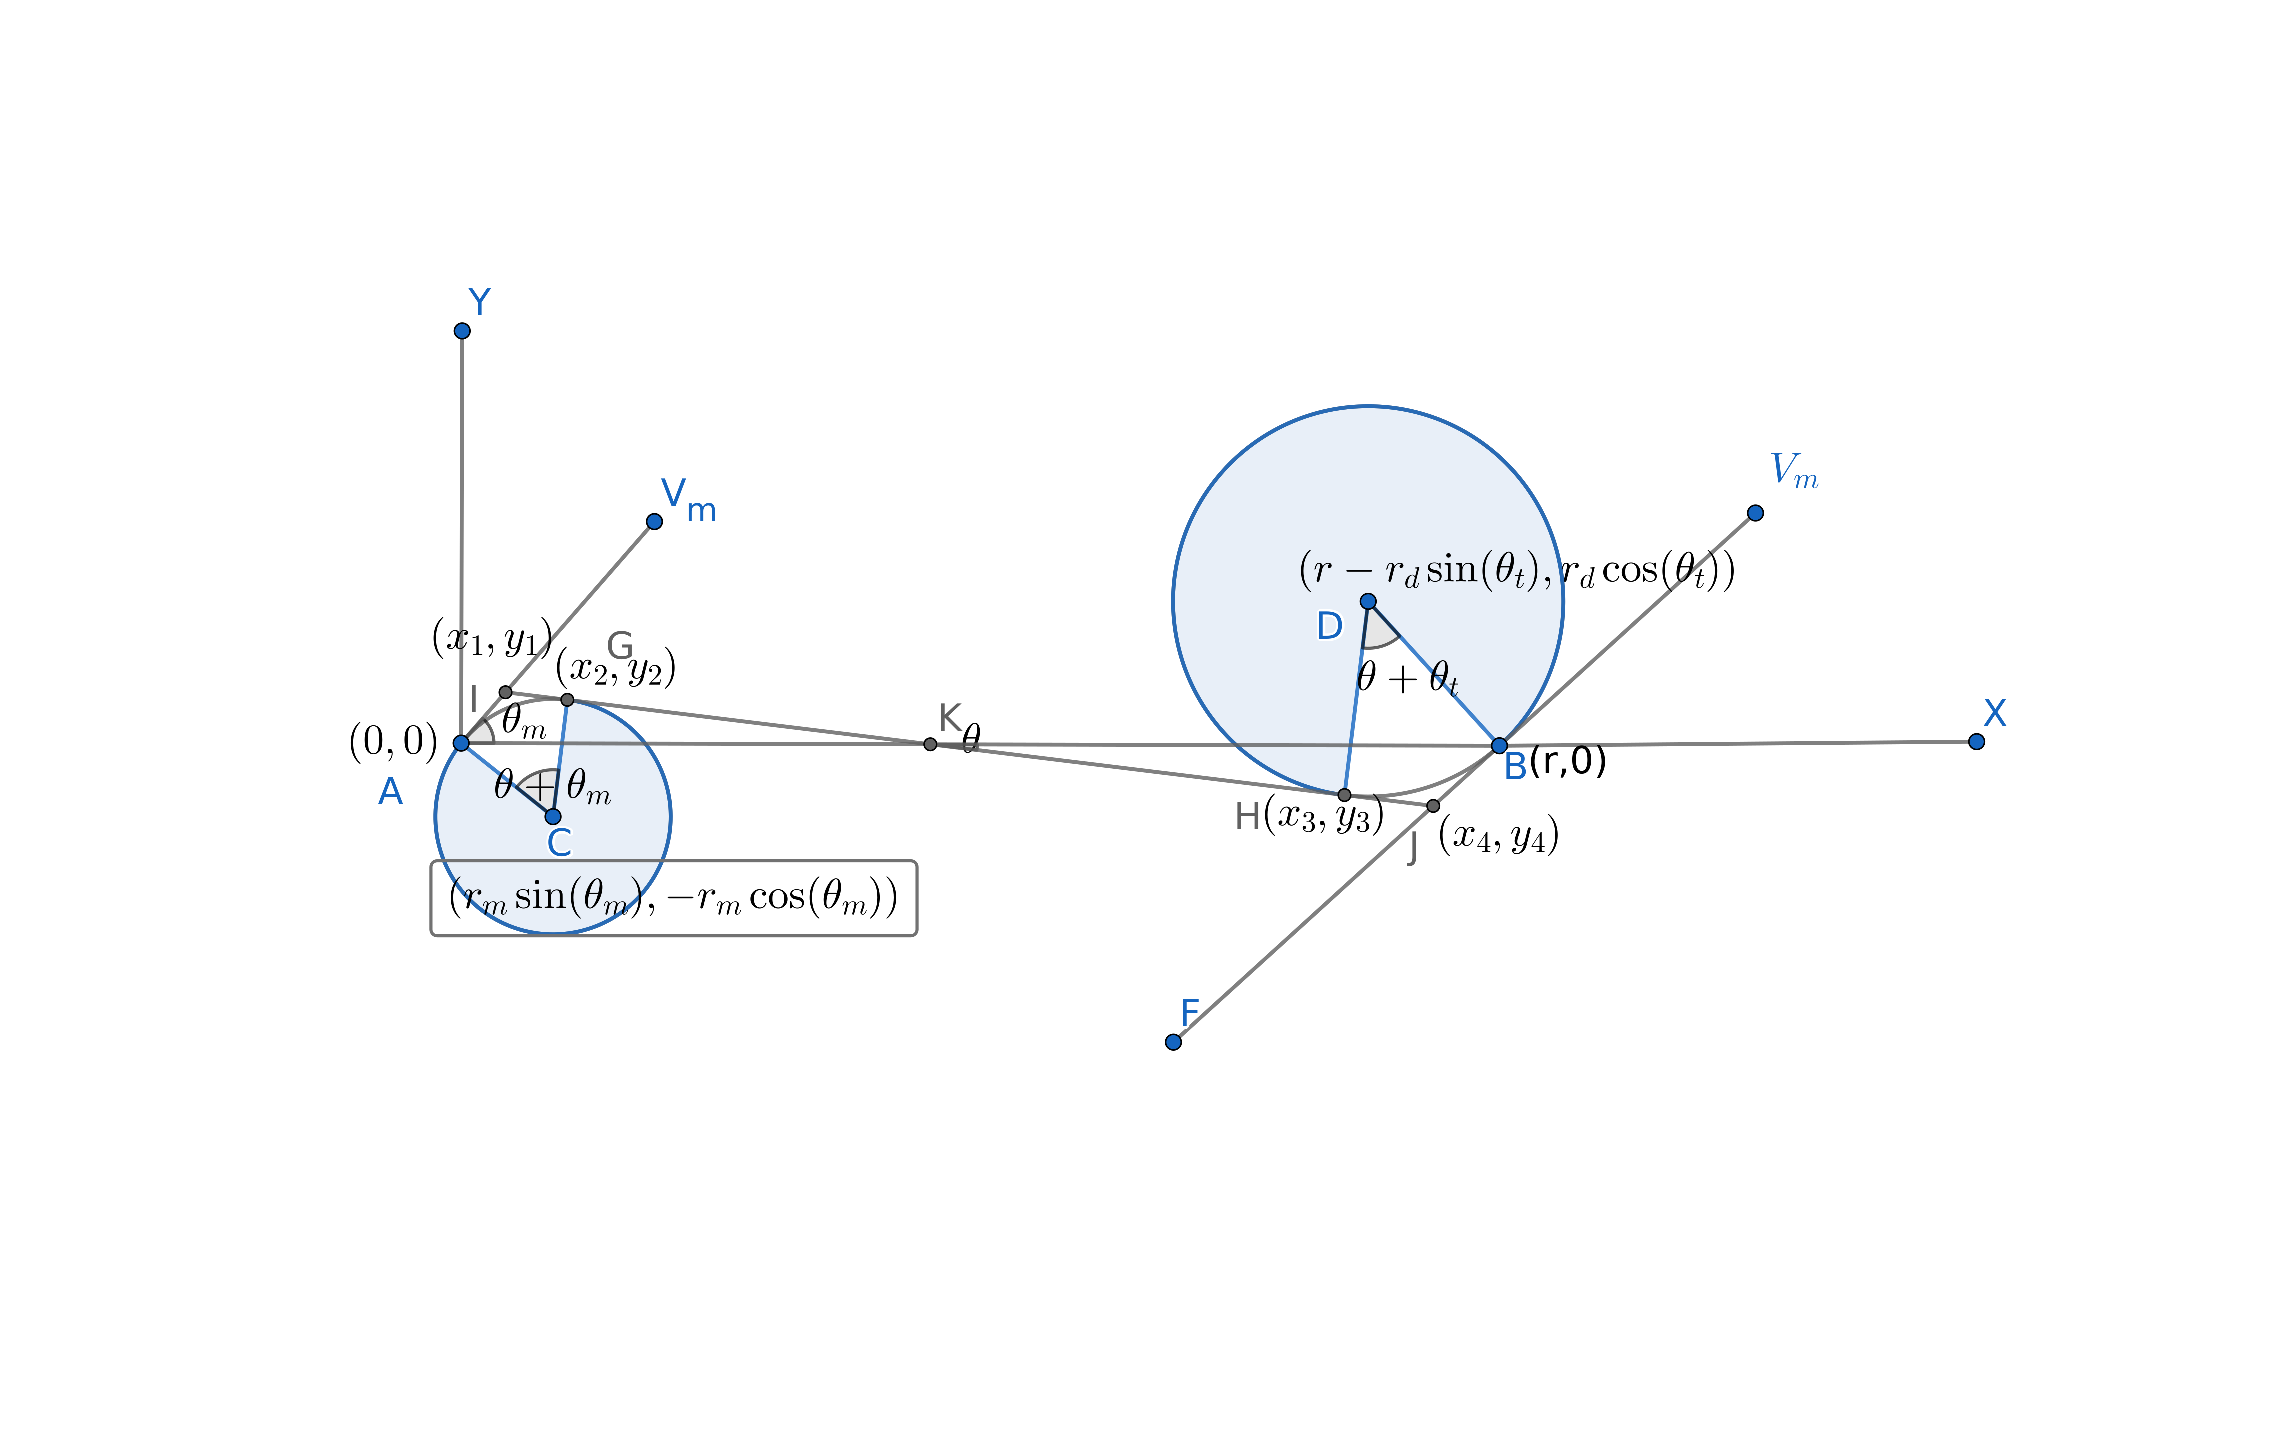
\includegraphics[trim={5cm 6cm 7cm 4cm},clip,width=0.6\textwidth, keepaspectratio]{Images/TCT_final.eps}
		%\caption{The TCT-based Dubins-like path with same-sign angles}
	\end{figure}
	\vspace{-0.3cm}
	\begin{columns}[T]
		\begin{column}{0.45\textwidth}
			%\column{0.45\textwidth}
			Interceptor position - $(0,0)$ \\
			Target position - $(r,0)$\\ 
			Launch angle - $\theta_m \in (0,\pi)$
		\end{column}
		\vrule{}
		\begin{column}{0.5\textwidth}
			%\column{0.5\textwidth}
			Desired impact angle - $\theta_t \in (0,\pi)$ \\
			Scenario with $\theta_m \in (-\pi,0)$\\
			Length IG=$L_{t1}$ and HJ=$L_{t2}$
		\end{column}
	\end{columns}
	\vspace{0.2cm}
	\centering
	$\color{olive}r_{crit}^{TCT}=\frac{r^2-2rr_m\sin\theta_m}{2r_m(1-\cos(\theta_m-\theta_t)+2r\sin\theta_t)} \geq r_d \geq r_m =\frac{V_m^2}{a_{max}}$ \\
\end{frame}
%%%%%%%%%%%%%%%%%%%%%%%%%%%%%%%%%%%%%%%%%%%%%%%%%%%%%%%%%%%%%%%%%%%%%%%%%%%%%%%%%%%%%%%%%%%%%
\begin{frame}{TCT Based Path Planning - Derivation}
	Total path length (P) is $$\color{cyan}r_m(\theta_m+\theta)+\color{magenta}\frac{r-L_{t1}(\cos \theta_m+\cos \theta)-L_{t2}(\cos \theta_t+\cos \theta)}{\cos \theta}+ \color{brown}r_d(\theta_t+\theta)=\color{blue}f(\theta)$$
	\begin{itemize}
		\item $r_d=L_{t2}\cot \frac{\theta_t+\theta}{2}$
		\item $L_{t1}=\frac{c}{\tan \theta_m+\tan \theta}\sec\theta_m$ and $L_{t2}=\frac{c-r\tan \theta}{\tan \theta_t+\tan \theta}\sec\theta_t$
		\item $c=r_m(\cos \theta -\cos \theta_m+\sin \theta \tan \theta+\sin \theta_m \tan \theta)$
	\end{itemize}
	\begin{alertblock}{}
		Given impact time or path length, we can calculate $\theta$ and thus the design parameter $r_d$. \\
		\centering{Is  function $f$ Invertible ?}
	\end{alertblock}
\end{frame}
%%%%%%%%%%%%%%%%%%%%%%%%%%%%%%%%%%%%%%%%%%%%%%%%%%%%%%%%%%%%%%%%%%%%%%%%%%%%%%%%%%%%%%%%%%%%%
\begin{frame}{Path Uniqueness}
	\begin{figure}
		\centering
		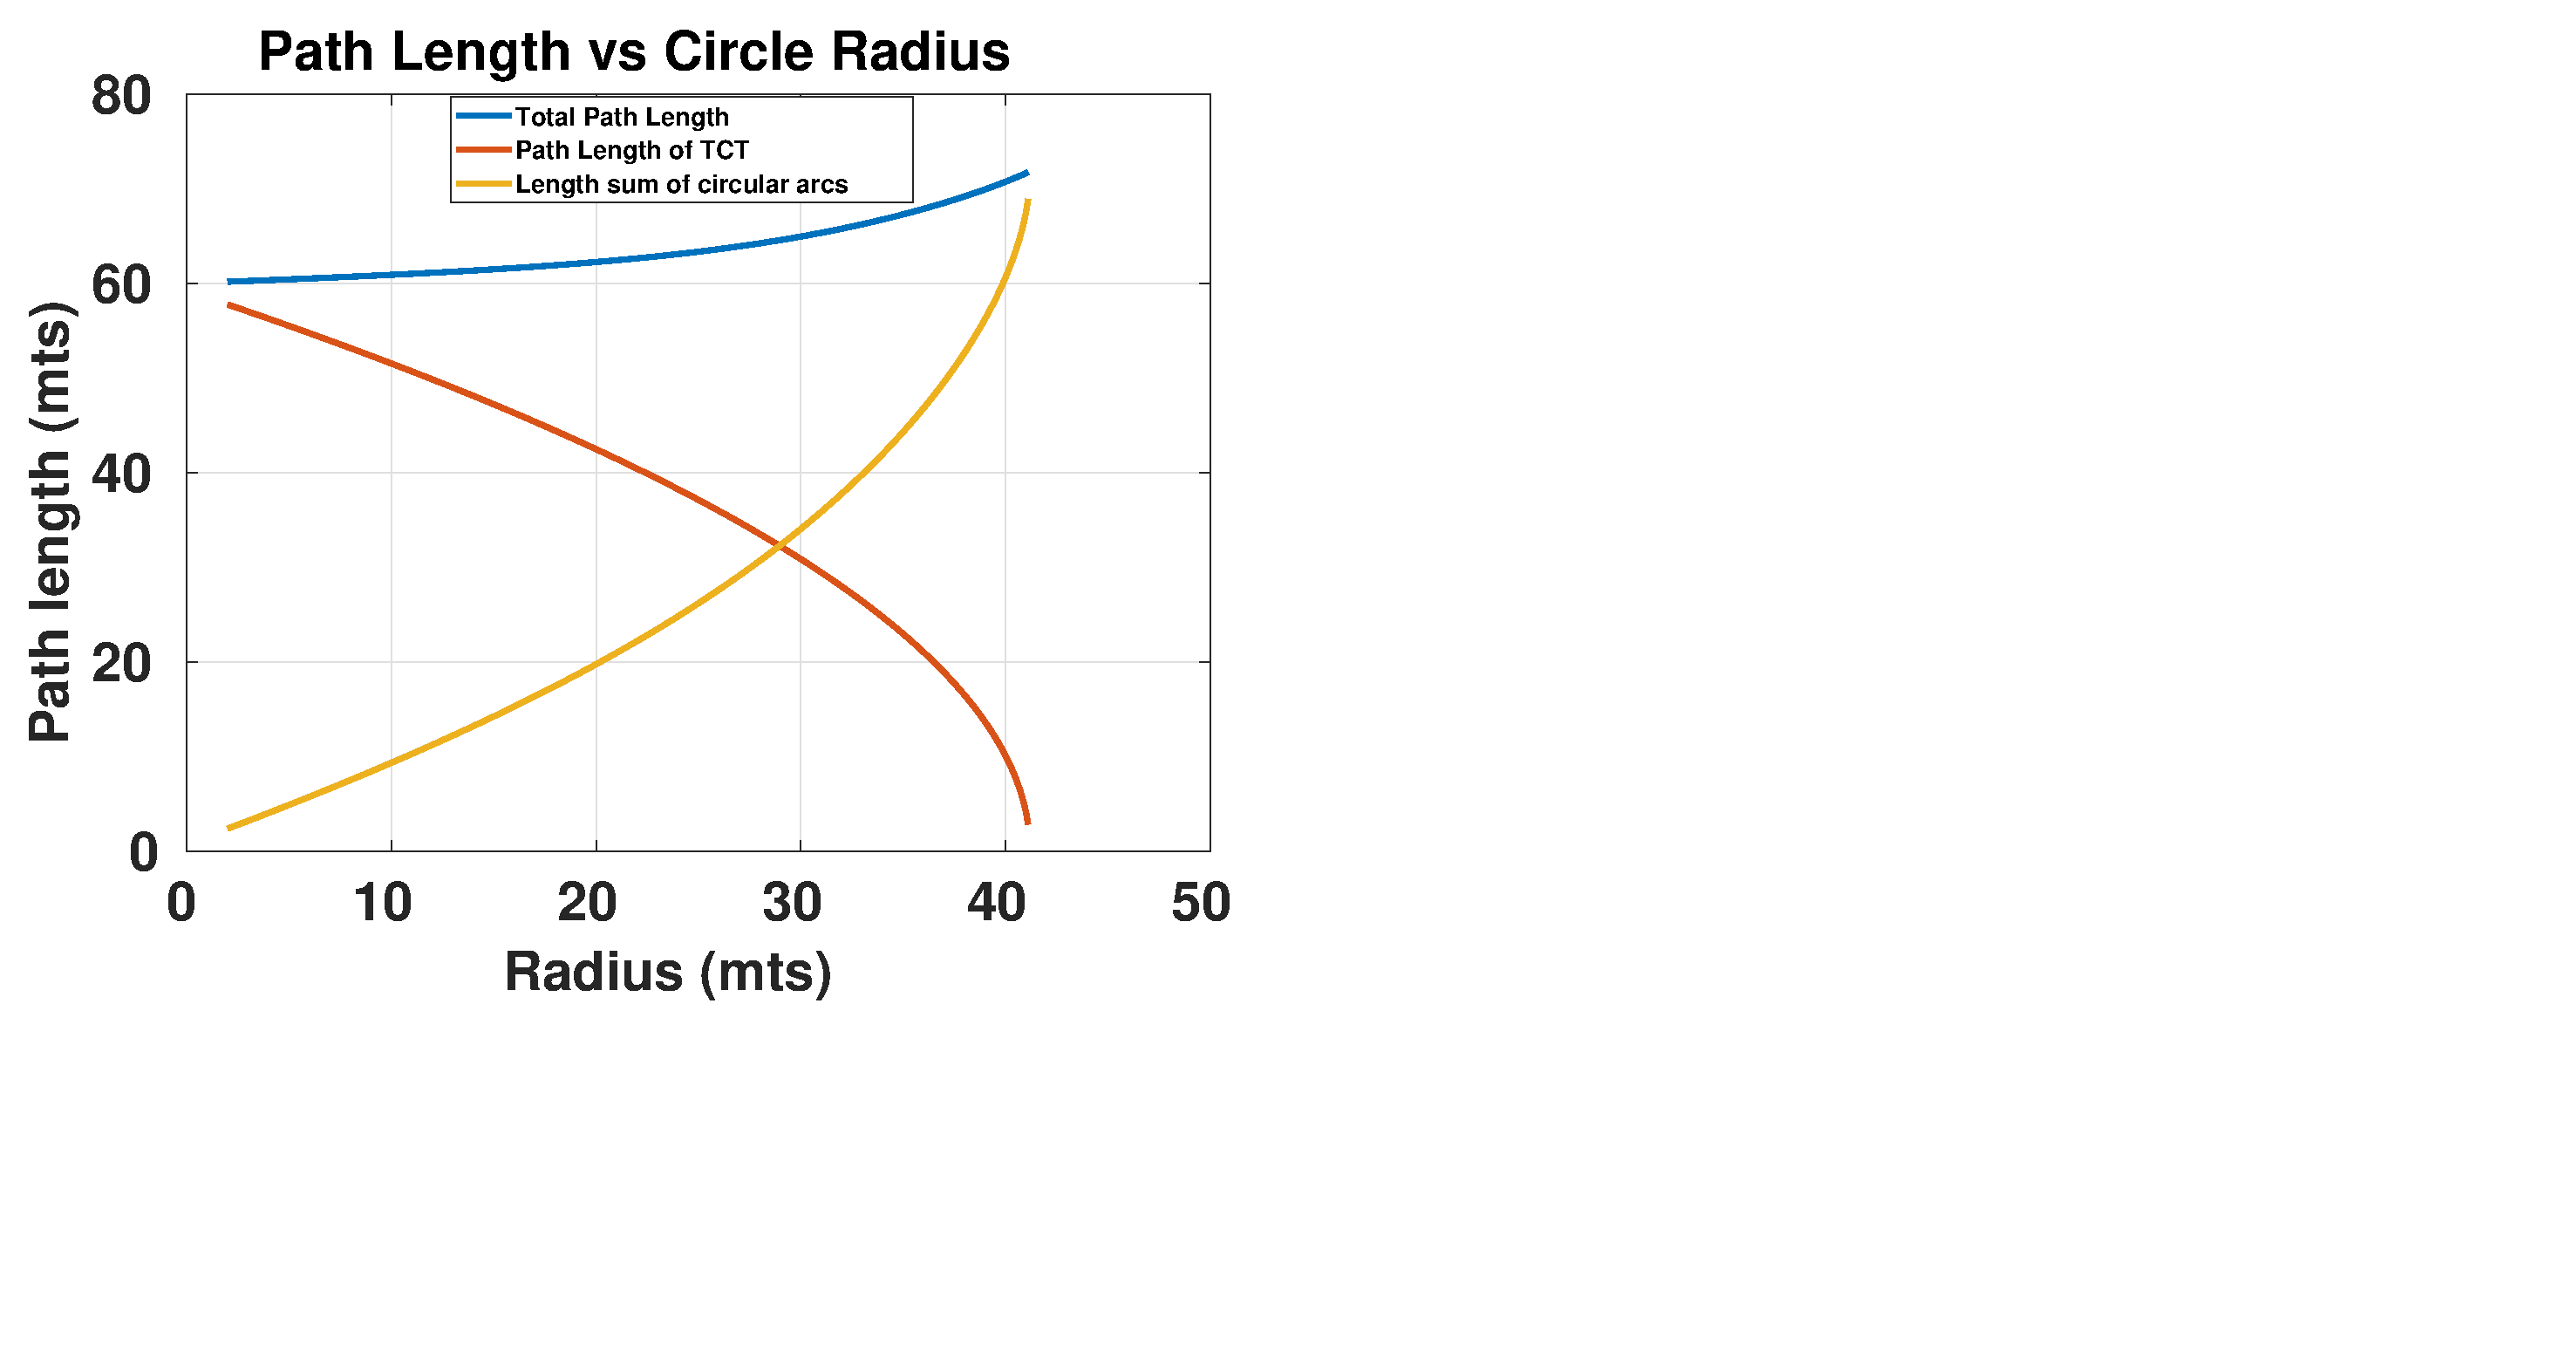
\includegraphics[trim={0cm 6cm 25cm 0cm},clip,scale=0.3]{Images/RadiusVsPathLength1.eps}%{newrad.eps}%
		%\caption{Path length vs radius [$r_d \in (r_m,r_{crit}^{TCT})$]}
		%\label{lengthvsradius}
	\end{figure}
	\vspace{-0.5cm}
	%\begin{block}{Note:}    
	\begin{itemize}
		\item TCT decreases
		\item Arc lengths increases 
		\item Total length Increases
	\end{itemize}
	%\end{block}
\end{frame}
%%%%%%%%%%%%%%%%%%%%%%%%%%%%%%%%%%%%%%%%%%%%%%%%%%%%%%%%%%%%%%%%%%%%%%%%%%%%%%%%%%%%%%%%%%%%%
\begin{comment}
\begin{frame}{TCT Based Path Planning- II}
	\begin{figure}
		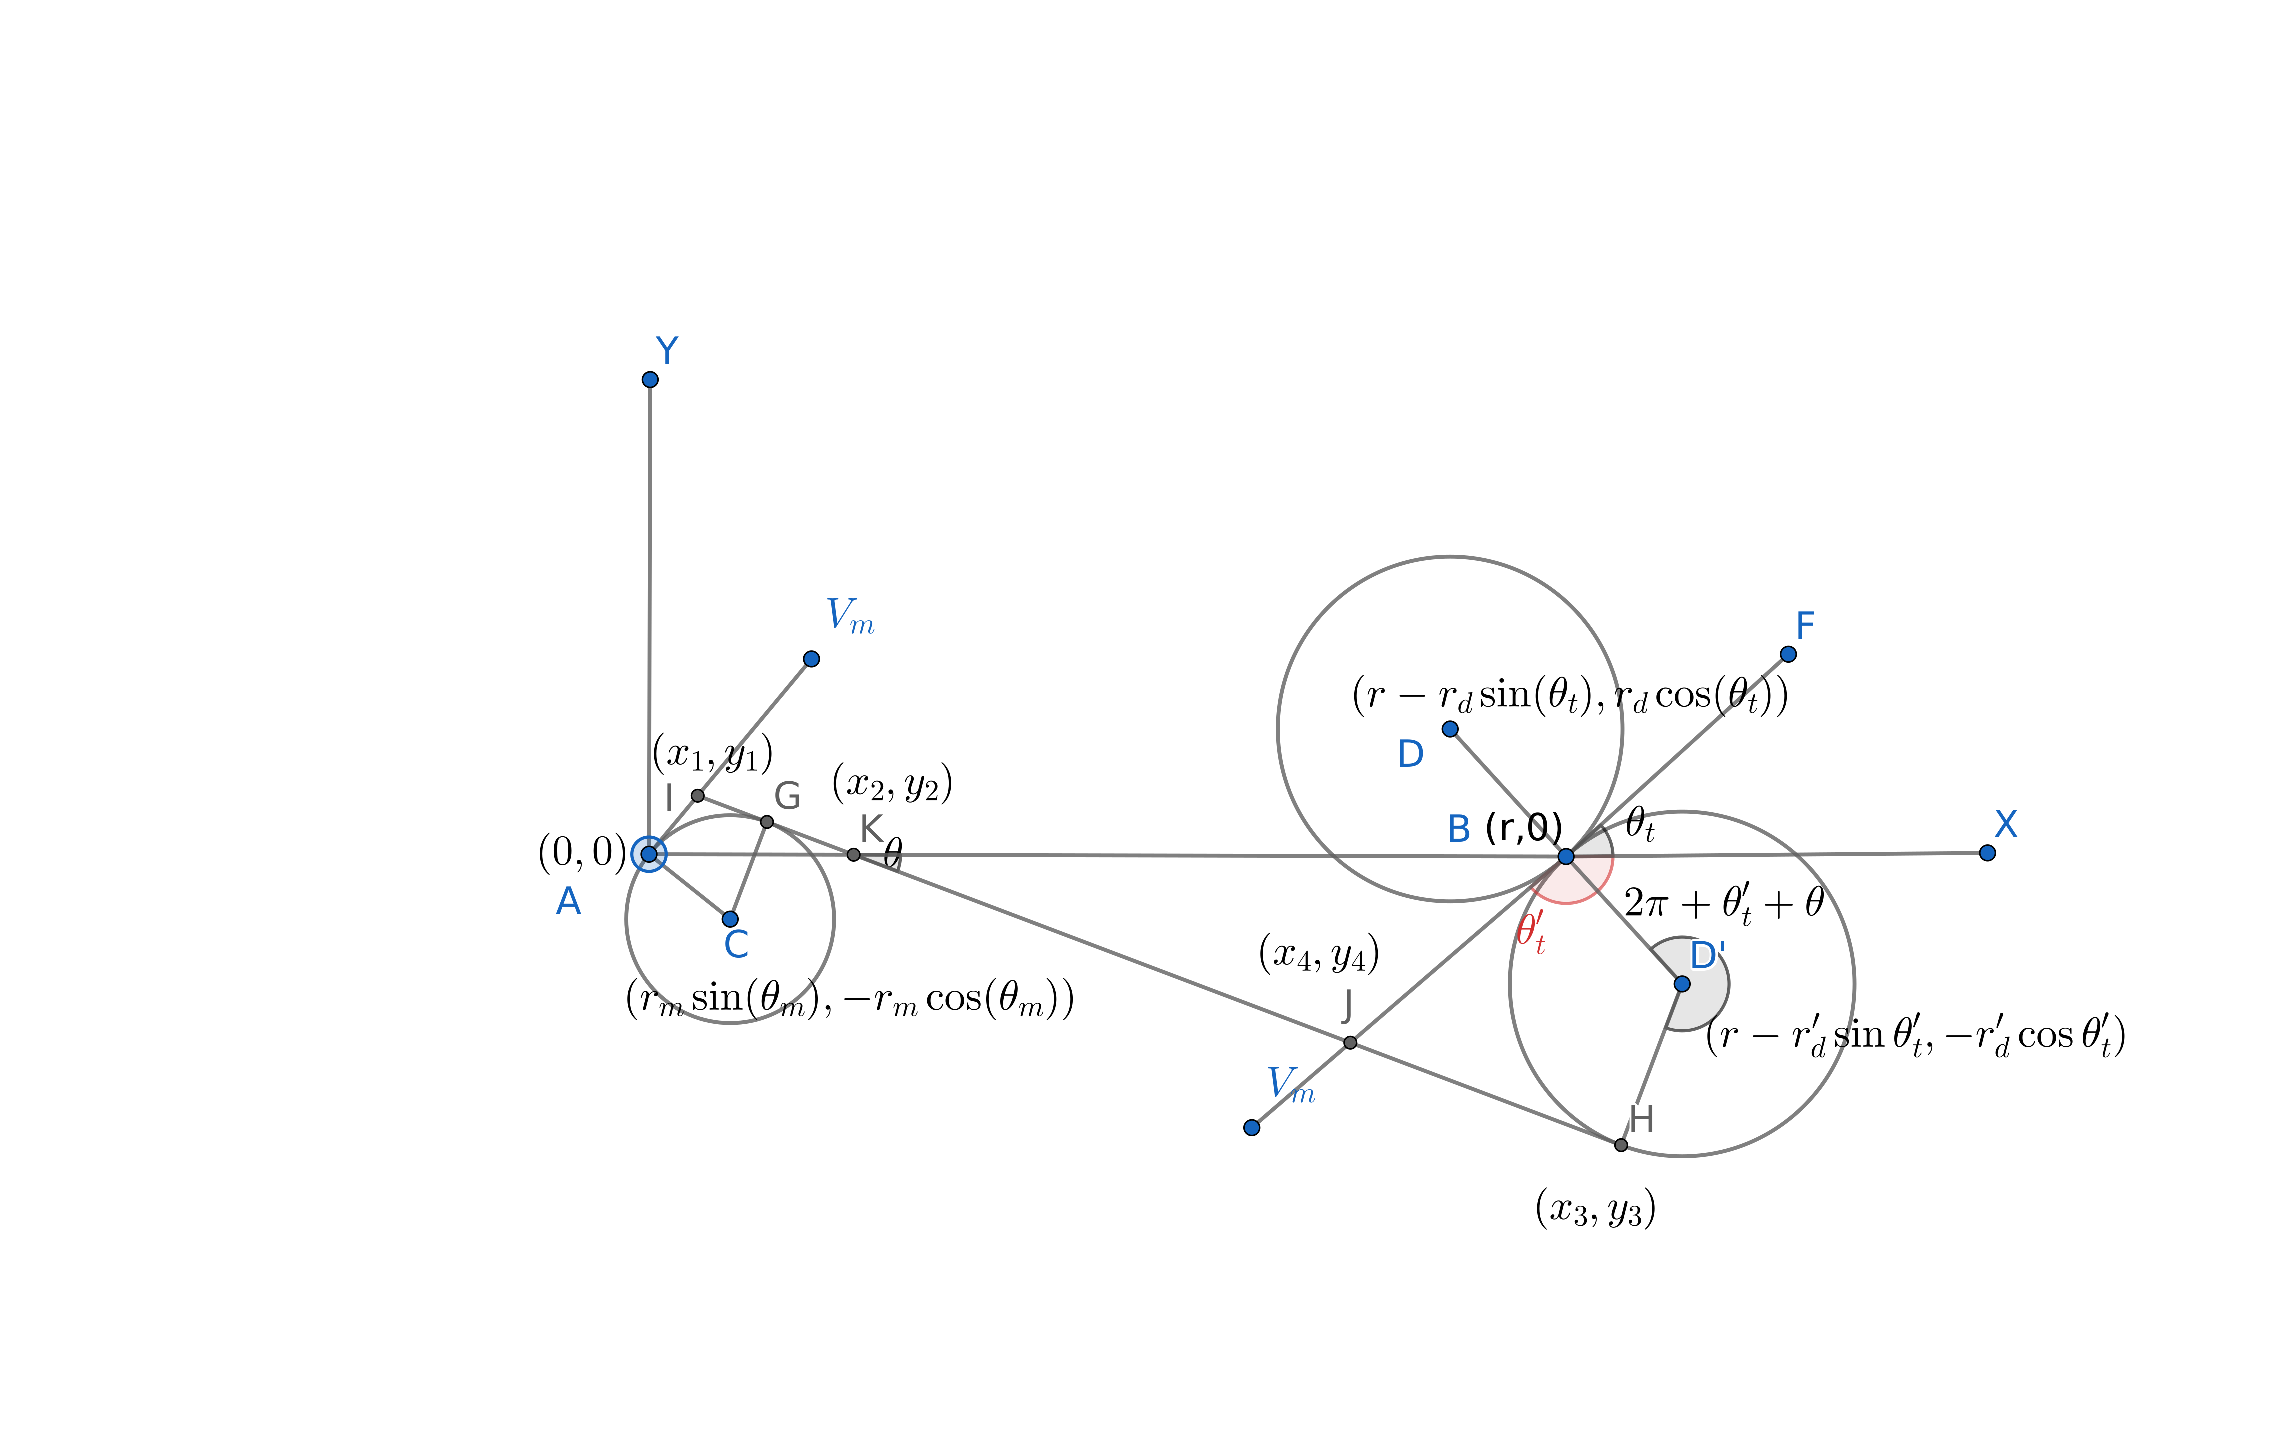
\includegraphics[trim={9cm 2.5cm 2cm 5cm},clip,width=0.7\textwidth]{Images/TCT_EXternal_Final.eps}
		%\caption{The TCT based Dubins like path when both the impact angle and target angle have opposite sign.}
	\end{figure} 
	\vspace{-1cm}
	-- $\theta_t \in (-\pi,0)$ \\
	-- $r_d \in (r_m, \infty)$ \\
	-- If larger impact time is required 
\end{frame}

\end{comment}
%%%%%%%%%%%%%%%%%%%%%%%%%%%%%%%%%%%%%%%%%%%%%%%%%%%%%%%%%%%%%%%%%%%%%%%%%%%%%%%%%%%%%%%%%%%%%
\begin{frame}{Guidance Design} \label{Guidance_Law}
	\begin{block}{}
		The guidance command is proposed as
		\begin{equation*}\label{mainguide}
			a_M=\begin{cases}
				a^{\rm max}\text{sgn}(x),~\text{for}~ 0<t<t_1,\\
				0~\text{for}~t_1<t<t_{1}+t_2\\
				\left(\dfrac{r_m}{r_d}\right)a^{\rm max}\text{sgn}(y)~\text{for}~t_1+t_2<t<t_{1}+t_2+t_3,
			\end{cases}
		\end{equation*}
		-- $t_1,t_1+t_2,t_1+t_2+t_3$ - switching time instants (in seconds)\\
		-- $\text{sgn}(\cdot)$ - the signum function. \\
		-- $x$ and $y$ - arbitrary non-zero real numbers whose signs are opposite.   
	\end{block}
\hyperlink{Dubin_based_Simulation}{\beamerbutton{Simulations}}
\end{frame}

\begin{frame}{Conclusion And Future Work}
	\begin{block}{Conclusion}
		\begin{itemize}
			\item Proposed a simple to implement guidance strategy using piece wise linear accelerations only.
			\item Simultaneously satisfied both the terminal constraints namely Impact Angle and Time.
			\item It was established that launching a vehicle with negative direction to the desired impact angle is advantageous.
		\end{itemize}
	\end{block}
	\textcolor{blue}{Publications: }\\
	\begin{enumerate}
		\item Dubey, A. K., Mukherjee, D., \& Kumar, S. R. (2024, June). Trajectory Planning Using Dubins-Like Paths with Approach Angle and Terminal Time Constraints. In 2024 32nd Mediterranean Conference on Control and Automation (MED) (pp. 412-417). IEEE.
	\end{enumerate}	
\end{frame}

%%%%%%%%%%%%%%%%%%%%%%%%%%%%%%%%%%%%%%%%%%%%%%%%%%%%%%%%%%%%%%%%%%%%%%%%%%%%%%%%%%%%%%%
\begin{subframe}{Simulation Setup}\label{Dubin_based_Simulation}
	\begin{columns}
		\begin{column}{0.5\textwidth}
			-- Desired impact angle $\theta_t=45^\circ$\\
			-- Impact time $t_{imp}=22\,\text{s}$\\
			-- Interceptor's speed $V_m=500\,\text{m/s}$    
		\end{column}
		\vrule{}
		\begin{column}{0.5\textwidth}
			-- Maximum lateral acceleration $a_{max}=400\,\text{m/s}^2$\\
			-- Launch angle $\theta_m=90^\circ$\\
			-- Initial range-to-go $r=10000\,\text{m}$
		\end{column}
	\end{columns}
	\begin{block}{}
		The closed-loop implementation of proposed strategy can be performed using 
		\begin{align}\label{mainguidecl}
			\nonumber a_M=&\frac{a^{\rm max}}{2}\left[\left\{1+\text{sign}(A_1-A)\right\}\text{sgn}(x)\right.\\
			\nonumber &\left.+\left(\frac{r_m}{r_d}\right) \left\{1-\text{sign}(A_1+\ell_{TCT}-A)\right\}\text{sgn}(y)\right], 
		\end{align}
		-- $A$ - Distance (length of the path) traveled by the interceptor since its launch \\
		-- $A_1$ - Distance travelled on circle 1 \\
		-- $\ell_{TCT}$ - Distance travelled on straight line.
	\end{block}
	
\end{subframe}
%%%%%%%%%%%%%%%%%%%%%%%%%%%%%%%%%%%%%%%%%%%%%%%%%%%%%%%%%%%%%%%%%%%%%%%%%%%%%%%%%%%%%%%
\begin{subframe}{Impact Angle $45^\circ$ And Impact Time $22s$}
	\begin{figure}
		%\subfigure[Trajectories.]{\includegraphics[scale=0.75]{trajakd.eps}\hspace{-.2cm}
			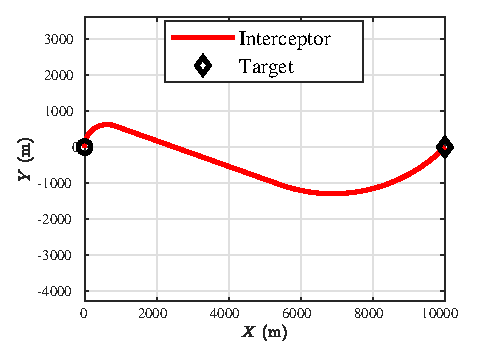
\includegraphics[scale=0.75]{Images/trajakd.eps}
			%\subfigure[$a_M$ and heading angle.]{\includegraphics[scale=0.75]{amsigmakd.eps}
				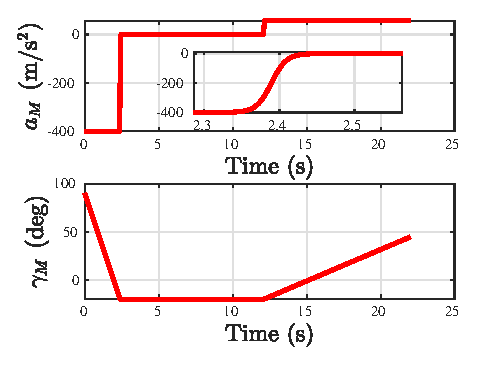
\includegraphics[scale=0.75]{Images/amsigmakd.eps}
				%\caption{Interception of stationary target using TCT at an impact angle of $45^\circ$ and an impact time of 22 seconds.}
	\end{figure}
	\begin{alertblock}{}
				The proposed guidance strategy works for $\theta_m=90^\circ$, whereas, this is not true for many guidance strategies. 
	\end{alertblock}
\end{subframe}
%%%%%%%%%%%%%%%%%%%%%%%%%%%%%%%%%%%%%%%%%%%%%%%%%%%%%%%%%%%%%%%%%%%%%%%%%%%%%%%%%%%%%%%
\begin{subframe}{Impact Angle $45^\circ$ And Different Impact Times}
			\begin{figure}
				%\subfigure[Trajectories.]{\includegraphics[scale=0.55]{traj_tct_compakd.eps}}\hspace{-.2cm}
				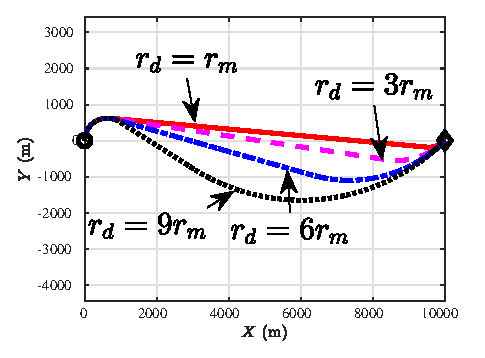
\includegraphics[scale=0.75]{Images/traj_tct_compakd.eps}
				%\subfigure[$a_M$ and heading angle.]{\includegraphics[scale=.23]{amgammam_tct_compsrk.eps}}
				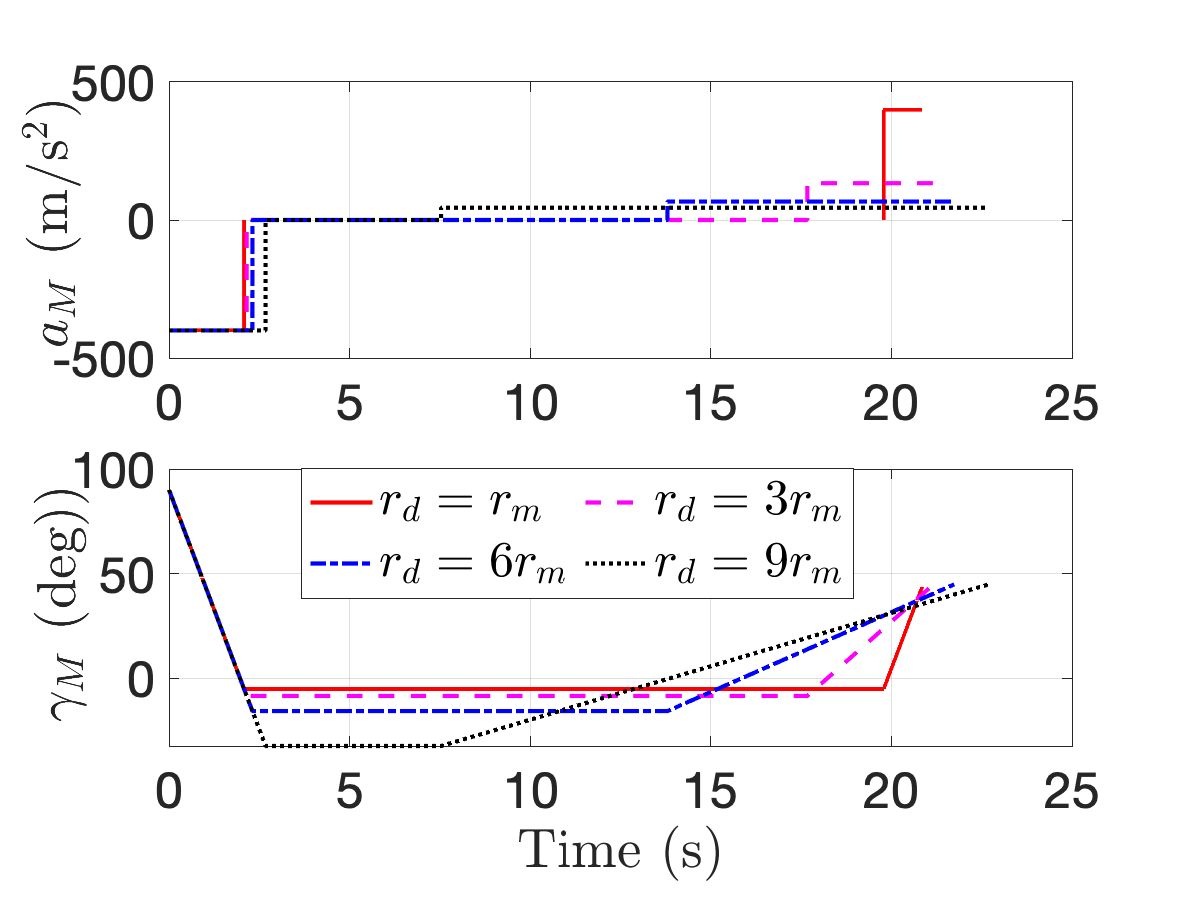
\includegraphics[scale=.3]{Images/amgammam_tct_compsrk.eps}
				%\caption{Interception of stationary target using TCT at an impact angle of $45^\circ$ with different impact times.}
			\end{figure}
\end{subframe}
%%%%%%%%%%%%%%%%%%%%%%%%%%%%%%%%%%%%%%%%%%%%%%%%%%%%%%%%%%%%%%%%%%%%%%%%%%%%%%%%%%%%%%%
\begin{subframe}{Impact Angle $45^\circ$ And Different Impact Times: TCT II}
			\begin{figure}
				\centering
				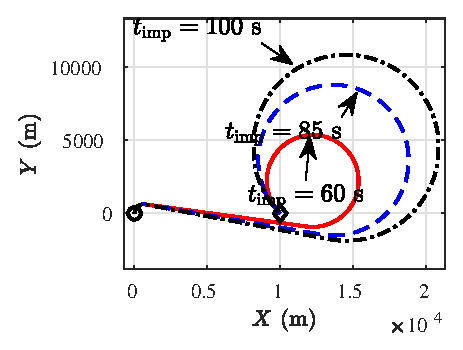
\includegraphics[scale=0.95]{Images/traj_out_tct1akd.eps}
				%\caption{Interception of stationary target using TCT at an impact angle of $45^\circ$ with different impact times when target angle is negative.}
			\end{figure}
			\vspace{-0.5cm}
			\begin{alertblock}{Note:}
				The impact time is unbounded when launched in a direction opposite to the desired impact angle using TCT based approach. 
			\end{alertblock}
\end{subframe}
%%%%%%%%%%%%%%%%%%%%%%%%%%%%%%%%%%%%%%%%%%%%%%%%%%%%%%%%%%%%%%%%%%%%%%%%%%%%%%%%%%%%%%%
\begin{subframe}{Comparison With Existing Strategies}\hyperlink{Guidance_Law}{\beamerbutton{Back2Guidance}}
			\vspace{-0.5cm}
			\begin{figure}
				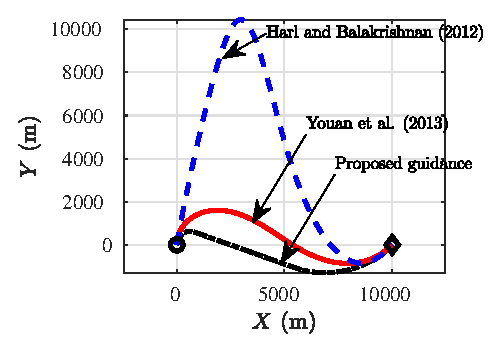
\includegraphics[scale=0.73]{Images/traj_compakd.eps}\hspace{.2cm}
				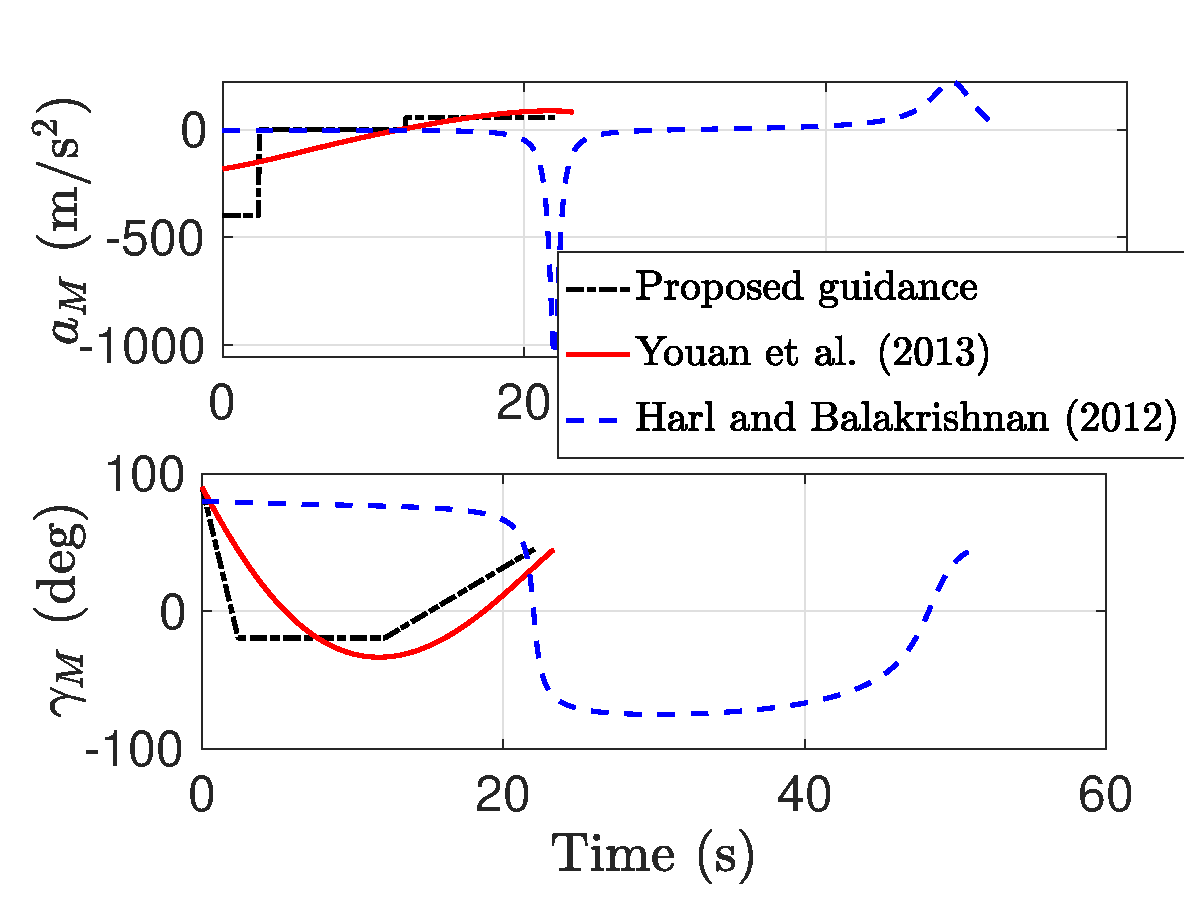
\includegraphics[scale=.3]{Images/am_comp_dubsrk.eps}	
				%\caption{Comparison with existing guidance strategies for an impact angle of $\mp 45^\circ$ and impact time of 22 seconds.}
			\end{figure}
			\vspace{-0.25cm}
			\begin{columns}
				\begin{column}{0.48\textwidth}
					-- \textit{Youan e. al (2013)}\footnotemark[1] 
					\begin{itemize}
						\item Succeeds to intercept when launched at $90^\circ$\\
						\item Exceeds the time requirements.
					\end{itemize}
				\end{column}
				\vrule{}
				\begin{column}{0.52\textwidth}
					-- \textit{Harl And Balakrishnan (2012)}\footnotemark[2]
					\begin{itemize}
						\item Fails to intercept when launched at $90^\circ$\\
						\item $\theta_M=80^\circ$, high impact time.
					\end{itemize}
				\end{column}
			\end{columns}
			\vspace{0.1cm}
			\footnotetext[1]{Zhang, Youan, Guoxin Ma, and Aili Liu. "Guidance law with impact time and impact angle constraints." Chinese Journal of Aeronautics 26.4 (2013): 960-966.}
			\footnotetext[2]{Harl, Nathan, and Sivasubramanya Nadar Balakrishnan. "Impact time and angle guidance with sliding mode control." IEEE Transactions on control systems technology 20.6 (2011): 1436-1449.}

\end{subframe}
%%%%%%%%%%%%%%%%%%%%%%%%%%%%%%%%%%%%%%%%%%%%%%%%%%%%%%%%%%%%%%%%%%%%%%%%%%%%%%%%%%%%%%%
\begin{comment}
	\begin{frame}{Simulation: Variation of the Lateral Acceleration and Impact Time}
		\begin{block}{Future Work}
			\begin{itemize}
			\item To obtain a closed loop implementation
			\item To extend it to multi-body problem for salvo attack.
			\end{itemize}
		\end{block}
				-- $\lambda_{P0}=\pi \quad r_{P0}=100\text{m} \quad V_P=500\,\text{m/s}$\\
				-- For $2000$ pairs $(\zeta_P,p)$ distributed uniformly over grid $[-\pi,\pi]\times[0.1, 1]$
				\vspace{-0.9cm}
				\begin{columns}
					\begin{column}{0.3\textwidth}
						\begin{figure}
							\centering
							\includegraphics[scale=0.5]{Images/t_imp_with_params.eps}
						\end{figure}
					\end{column}
					\begin{column}{0.3\textwidth}
						\begin{figure}
							\centering
							\includegraphics[scale=0.5]{Images/t_imp_with_p.eps}
						\end{figure}
					\end{column}
					\begin{column}{0.3\textwidth}
						--  For a fixed $\zeta_p$, $t_{imp} \downarrow$ when $p \uparrow$
					\end{column}
				\end{columns}
				\vspace{-0.9cm}
				\begin{columns}
					\begin{column}{0.3\textwidth}
						\begin{figure}
							\centering
							\includegraphics[scale=0.5]{Images/a_pmax_with_params.eps}
						\end{figure}
					\end{column}
					\begin{column}{0.3\textwidth}
						\begin{figure}
							\centering
							\includegraphics[scale=0.5]{Images/a_pmax_with_p.eps}
						\end{figure}
					\end{column}
					\begin{column}{0.3\textwidth}
						-- For a fixed $\zeta_p$, U-shaped $a_{P,\max}$ suggests the existence of an optimal trajectory that minimizes the lateral acceleration required.\\
						-- Minima is itself a function of $\zeta_P$\\
						-- No analytical expression for this optimal $p$ exists
					\end{column}
				\end{columns}
	\end{frame}			
\end{comment}
		
		
		
		
		
		
		
		%%%%%%%%%%%%%%%%%%%%%%%%%%%%%%%%%%%%%%%%%%%%%%%%%%%%%%%%%%%%%%%%%%%%%%%%%%%%%%%%%%%%%%%%%%%%%%%%%%%%%%%%
		
